\documentclass[a4paper,11pt]{article}
\input{/home/tof/Documents/Cozy/latex-include/preambule_lua.tex}
\newcommand{\showprof}{show them}  % comment this line if you don't want to see todo environment

\fancyhead[L]{Paradigmes de programmation - POO}
\newdate{madate}{10}{09}{2020}
\fancyhead[R]{Terminale - NSI} %\today
\fancyfoot[L]{~\\Christophe Viroulaud}
\fancyfoot[C]{\textbf{Page \thepage}}
\fancyfoot[R]{\includegraphics[width=2cm,align=t]{/home/tof/Documents/Cozy/latex-include/cc.png}}

\begin{document}
\begin{Form}
\paragraph{Objectif:}Différencier et utiliser plusieurs paradigmes de programmation.
\section{Problématique: Fortnite}
Chaque combattant de Fortnite est extrêmement personnalisable. C'est une des caractéristiques qui fait le succès du jeu.\\Il est ainsi possible de choisir les éléments: outfit, glider, contrail, back bling, emote, pickaxe, toy.

\begin{table}[!h]
\begin{tabular}{*{4}{>{\centering\arraybackslash}m{.23\textwidth}}}
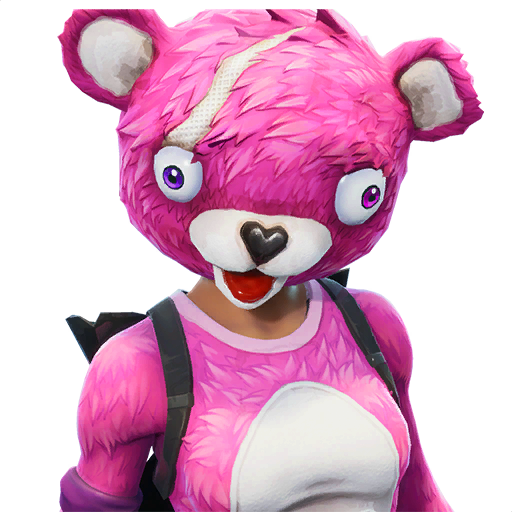
\includegraphics[width=3cm]{ressources/outfits/cuddle-team-leader.png} 
& 
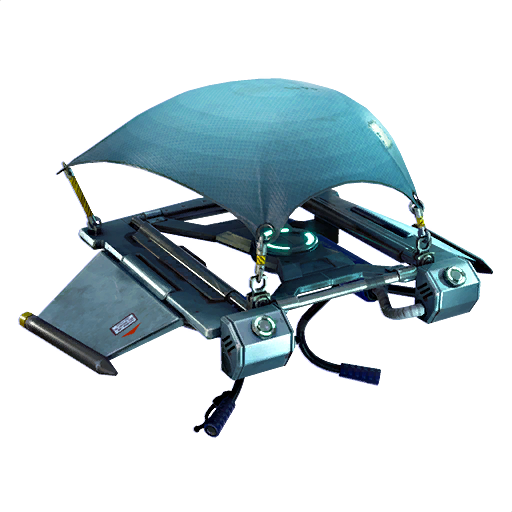
\includegraphics[width=3cm]{ressources/gliders/glider.png} 
&

\includegraphics[width=3cm]{ressources/emotes/disco-fever.png} 
&
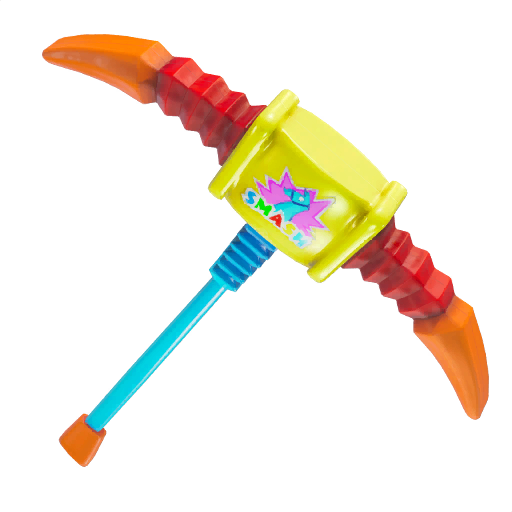
\includegraphics[width=3cm]{ressources/pickaxes/pick-squeak.png} 
 \\ 
 outfit & glider & emote & pickaxe \\
\end{tabular}
\caption{Exemples d'éléments}
\end{table}
Il faut ajouter à cela les objets récupérés en cours de partie et gérer l'évolution de l'énergie et du bouclier du personnage.

\begin{center}
\shadowbox{\parbox{12cm}{\centering Quel concept de programmation mettre en place pour manipuler les combattants et les faire évoluer dans une partie?}}
\end{center}
\section{Un concept déjà utilisé: paradigme impératif}
\begin{commentprof}
\subsection*{Retour historique}
Un paradigme de programmation est un style de programmation informatique qui traite de la manière dont les solutions aux problèmes doivent être formulées dans un langage de programmation.\\
La programmation impérative (du latin imperare: ordonner) est une séquence ordonnée d'instructions, fournies à l'ordinateur. premiers programmes = bas niveau = instructions aux plus proches de la machine (lis cette adresse mémoire...). Programmation impérative se calque sur le schéma de fonctionnement des ordinateurs (Von Neumann voir cours 1ere).\\1951: Grace Hopper 1° compilateur (A-0) = traduire programme en langage machine, puis langage Cobol en 1959 (programme doit être calqué sur langage humain plutôt que machine)\\1954: FORTRAN FORmula TRANslator; reste encore très utilisé (même si remplacé par C, C++) car nombreuses bibliothèques, coût important pour les remplacer, performant.\\1991: Fortran 90: modernisation, modules, récursivité\\1963: BASIC: dérivé du Fortran pour les débutants, l'apprentissage; mais trop simple, maintenance difficile; Djikstra écrit article assassin; fait disparaître au profit du Pascal\\1970: Pascal; écrit par Niklaus Wirth; très rapide car travaillant principalement en mémoire vive; Turbo Pascal dans les années 80.\\1972: C; crée par Dennis Ritchie (B trop limité) pour dvp système UNIX; avec Ken Thomson.
\end{commentprof}
\subsection{Stocker les informations}
Différentes structures de données abordées en Première permettent de contenir les informations du combattant.
\begin{activite}
\begin{enumerate}
\item Proposer un type (construit) de données et construire la structure permettant de stocker les éléments qui composent un combattant.
\item Ajouter une structure permettant de stocker et gérer les objets du sac à dos.
\item Ajouter enfin deux variables exprimant l'énergie et le bouclier. Ces variables seront initialisées à \emph{100}.
\end{enumerate} 
\end{activite}
\begin{commentprof}
Itération sur un dictionnaire. Pas de garantie d'ordre (selon version de Python <3.7).\\\url{https://docs.python.org/fr/3/tutorial/datastructures.html#looping-techniques}
\end{commentprof}
\subsection{Modifier les informations}
Lors d'une partie le joueur peut ramasser des objets pour les mettre dans son sac. Il peut également subir des dégâts lors d'une attaque.
\begin{activite}
\begin{enumerate}
\item Implémenter une fonction \textbf{ramasser\_objet} qui ajoute un objet dans le sac s'il n'est pas plein (trois objets maximum). Cette fonction prendra un paramètre \emph{objet} de type \emph{string}.
\item Implémenter une fonction \textbf{subir\_attaque} qui prendra un paramètre \emph{degat} de type \emph{integer} et qui modifiera les caractéristiques \emph{shield} et \emph{energy} du combattant. 
\item Dans Fortnite chaque objet a également plusieurs propriétés. Construire un type construit de données qui stocke les caractéristiques des armes présentées.
\end{enumerate}
\end{activite}
\begin{commentprof}
ATTENTION à éviter les variables globales!
\end{commentprof}
\begin{commentprof}
\subsection*{Limites du paradigme}
Les fonctions définies influent sur le combattant, mais d'autres items du jeu évoluent également pendant la partie. Les armes par exemple ont un nombre de munitions variables, le parachute peut être ouvert ou fermé.\\De plus, comment donner une arme à chaque combattant? Le système se complexifie alors, d'où l'intérêt d'introduire un nouveau paradigme.
\end{commentprof}
\section{Une nouvelle approche: paradigme objet}
\begin{commentprof}
\subsection*{Retour historique}
Dvpt informatique = pb de + en + complexe à résoudre (\emph{abstraction})
\begin{itemize}
\item impératif pas forcément suffisant ou pratique
\item modélisation d'une application informatique sous la forme d’objets, ayant des propriétés et pouvant interagir entre eux. La modélisation orientée objet est proche de la réalité ce qui fait qu’il sera relativement facile de modéliser une application de cette façon.
\item De plus, les personnes non-techniques pourront comprendre et éventuellement participer à cette modélisation.
\end{itemize}
1960: SIMULA = plutôt introduction des concepts\\
1971: Les travaux de ces deux informaticiens ont ensuite influencé ceux d'Alan Kay, informaticien américain à l'origine du langage Smalltalk dans les années 70. A l'époque, Alan Kay travaillait au laboratoire PARC de Xerox en Californie. C'est dans ce même laboratoire qu'est apparu (en 1973) le premier ordinateur utilisant un système d'exploitation avec interface graphique, la Station Xerox Alto qui a ensuite inspiré le Mac Intosh, puis le système d'exploitation Windows de Microsoft. Il faut remarquer que les travaux d'Alan Kay portaient simultanément sur la conception d'interface graphique et la programmation objet. Cette nouvelle manière de programmer était pour lui une manière élégante de représenter informatiquement les interfaces graphiques. 
\end{commentprof}
\subsection{Décrire une classe}
\subsubsection{Définition}
Une \emph{classe} définit une nouvelle structure de données. Elle regroupe plusieurs composantes de natures différentes. Dans notre cas c'est le combattant. Chaque langage implémentant la programmation orienté objet défini une syntaxe propre. 
\begin{lstlisting}
class Combattant:
\end{lstlisting}
La classe peut être vue comme le squelette générique du combattant.
\begin{commentprof}
Les bonnes pratiques (PEP8 - Python Enhancement Proposals = propositions d'amélioration) conseillent de mettre une majuscule pour les noms de class.
\end{commentprof}
\subsubsection{Ajouter des attributs}
La fonction \emph{\_\_init\_\_} est appelée automatiquement quand nous créons un combattant. Chaque caractéristique est représentée par une variable propre à la classe: \emph{un attribut}.
\begin{lstlisting}
class Combattant:
	"""Crée un combattant avec ses caractéristiques propres"""
	def __init__(self,tenue,parachute,trainee):
		self.outfit=tenue
		self.glider=parachute
		self.contrail=trainee
\end{lstlisting}
\begin{commentprof}
Nous commençons ici avec seulement 3 attributs.\\
Remarquez l'utilisation du mot dédiée \emph{self} en Python. La syntaxe peut être différente dans d'autres langages (javascript = this, C++ = rien). Pourquoi \emph{self}? permet de faire référence explicite à l'instance de la classe en cours. Différencie variable locale des autres.\\Enfin on aurait pu initialiser les attributs dans un second temps et pas directement dans le \_\_init\_\_.
\end{commentprof}
\subsection{Créer un objet}
\subsubsection{Créer un combattant}
La classe est la structure (le squelette) d'un combattant. Pour l'instant aucun joueur n'a été construit. On crée une \emph{instance} de la classe \emph{Combattant} et on la stocke dans la variable \emph{joueur1}.
\begin{lstlisting}
joueur1=Combattant("cuddle-team-leader","hot-rod","flames")
\end{lstlisting}
\begin{activite}
\begin{enumerate}
\item Compléter la classe \emph{Combattant} en ajoutant toutes les caractéristiques.
\item Créer un nouvel attribut permettant de stocker le contenu du sac à dos.
\end{enumerate}
\end{activite}
\subsubsection{Manipuler les attributs}
Nous pouvons consulter les valeurs d'un attribut mais aussi les modifier.
\begin{lstlisting}
>>> joueur1.outfit
cuddle-team-leader
>>> joueur1.glider="pterodactyl"
\end{lstlisting}

\begin{commentprof}
En Python nous avons pouvons accéder à tout le contenu de la classe. Ce n'est pas le cas dans tous les langages: la POO est souvent associée à la notion \emph{d'encapsulation}. Le programmeur peut vouloir masquer le contenu d'implémentation. Par convention en Python les attributs privés sont précédés d'un \_.
\end{commentprof}
\subsection{Manipuler les données}
La manipulation de l'objet passe de préférence par une interface constituée de fonctions définies dans la classe: \emph{les méthodes}.
\begin{lstlisting}
class Combattant:
	"""Crée un combattant avec ses caractéristiques propres"""
	def __init__(self,tenue,parachute,trainee):
		self.outfit=tenue
		self.glider=parachute
		self.contrail=trainee
	
	def get_outfit(self):
		return self.outfit
	
	def set_outfit(self,nouvelle):
		self.outfit=nouvelle
\end{lstlisting}
\begin{commentprof}
getters (accesseurs) et setters (mutateurs)
\end{commentprof}
Dans le programme principal, le code ci-après affiche la tenue du combattant:
\begin{lstlisting}
joueur1.get_outfit()
\end{lstlisting}
\begin{activite}
\begin{enumerate}
\item Ajouter les attributs \emph{energy, shield} et \emph{backpack}.
\item Adapter les fonctions \emph{subir\_attaque} et \emph{ramasser\_objet} pour en faire des méthodes de la classe \emph{Combattant}.
\end{enumerate}
\end{activite}
\begin{commentprof}
Et Python dans tout ça; quel paradigme?
\end{commentprof}
\subsection{Le monde est objet}
\begin{activite}
\begin{enumerate}
\item Créer un objet \emph{Weapon} possédant les attributs présentés précédemment.
\item Ajouter une méthode \emph{tirer} qui vide une balle du magasin. Cette méthode renverra le texte \emph{Chargeur vide!} quand toutes les balles auront été tirées.
\item Implémenter une méthode \emph{recharger} qui remplit le magasin.
\end{enumerate}
\end{activite}
\begin{commentprof}
Comment gérer le nombre de balles à recharger? un attribut \emph{cachée} qui enregistre le nombre de balles à la création de l'arme.
\end{commentprof}
\end{Form}
\end{document}